\documentclass{beamer}
\usepackage[utf8]{inputenc}
\usepackage{graphicx}
\usepackage{tikz}
\usepackage{fontspec}
\usepackage{multirow}

% Clean theme
\usetheme{Madrid}
\usecolortheme{default}
\setbeamertemplate{navigation symbols}{}
\setbeamertemplate{footline}{}
\setbeamertemplate{headline}{}

% Typography — FiraSans (modern, readable sans-serif, close to SF Compact)
\usepackage[sfdefault]{FiraSans}
\renewcommand{\familydefault}{\sfdefault}

% Colors
\definecolor{darkblue}{RGB}{0, 102, 204}
\setbeamercolor{background canvas}{bg=white}
\setbeamercolor{title}{fg=darkblue}
\setbeamercolor{frametitle}{fg=darkblue}

\setbeamersize{text margin left=0.5cm, text margin right=0.5cm}

\title{Does Proximity Feedback Modality Reduce Falls in a Non-Dominant Hand Tilt Task?}
\subtitle{PathSense: A Preliminary Study}
\author{Eugene Sy}
\date{June 2, 2026}

\begin{document}

% ====== SLIDE 1: TITLE ======
\begin{frame}[plain]
  \vspace{2.5cm}
  \centering
  \textcolor{darkblue}{\Large \textbf{Does Proximity Feedback Modality}}

  \vspace{0.3cm}

  \textcolor{darkblue}{\Large \textbf{Reduce Falls in a Non-Dominant Hand}}

  \vspace{0.3cm}

  \textcolor{darkblue}{\Large \textbf{Tilt Task?}}

  \vspace{1.5cm}
  {\large PathSense: A Preliminary Study}

  \vspace{0.5cm}
  {\small Eugene Sy • June 2, 2026}
\end{frame}

% ====== SLIDE 2: THE PROBLEM (3 actual photos: everyday + surgical + precision) ======
\begin{frame}[plain]
  \vspace{0.3cm}
  \centering

  \textcolor{darkblue}{\Large \textbf{One Hand Busy, One Hand Blind}}

  \vspace{0.3cm}

  {\small \textit{Your brain can't control what it can't sense.} \\
  \small \textit{Elderly shopping $\cdot$ Surgical precision $\cdot$ Drone piloting: same principle.}}

  \vspace{0.4cm}

  \begin{columns}[T]
    \column{0.32\textwidth}
    \centering
    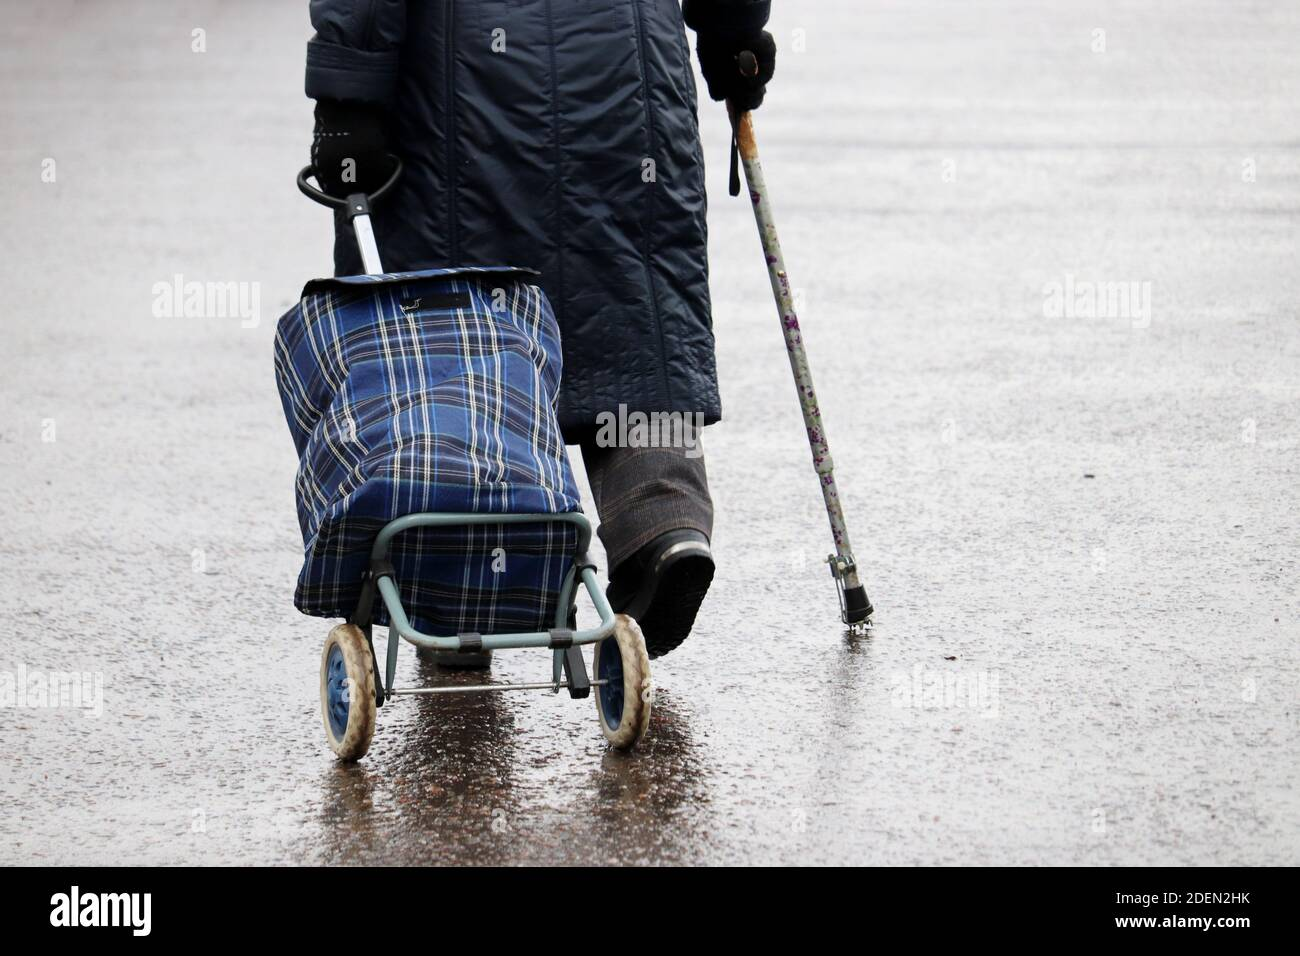
\includegraphics[width=0.95\textwidth]{images/elderly_shopping.jpg}
    \vspace{0.2cm}
    {\footnotesize \textbf{Everyday}}
    {\tiny Cane + shopping bag}

    \column{0.32\textwidth}
    \centering
    
\includegraphics[width=0.95\textwidth]{images/surgery_robot.jpg}
    \vspace{0.2cm}
    {\footnotesize \textbf{Surgical}}
    {\tiny Robotic arm precision}

    \column{0.32\textwidth}
    \centering
    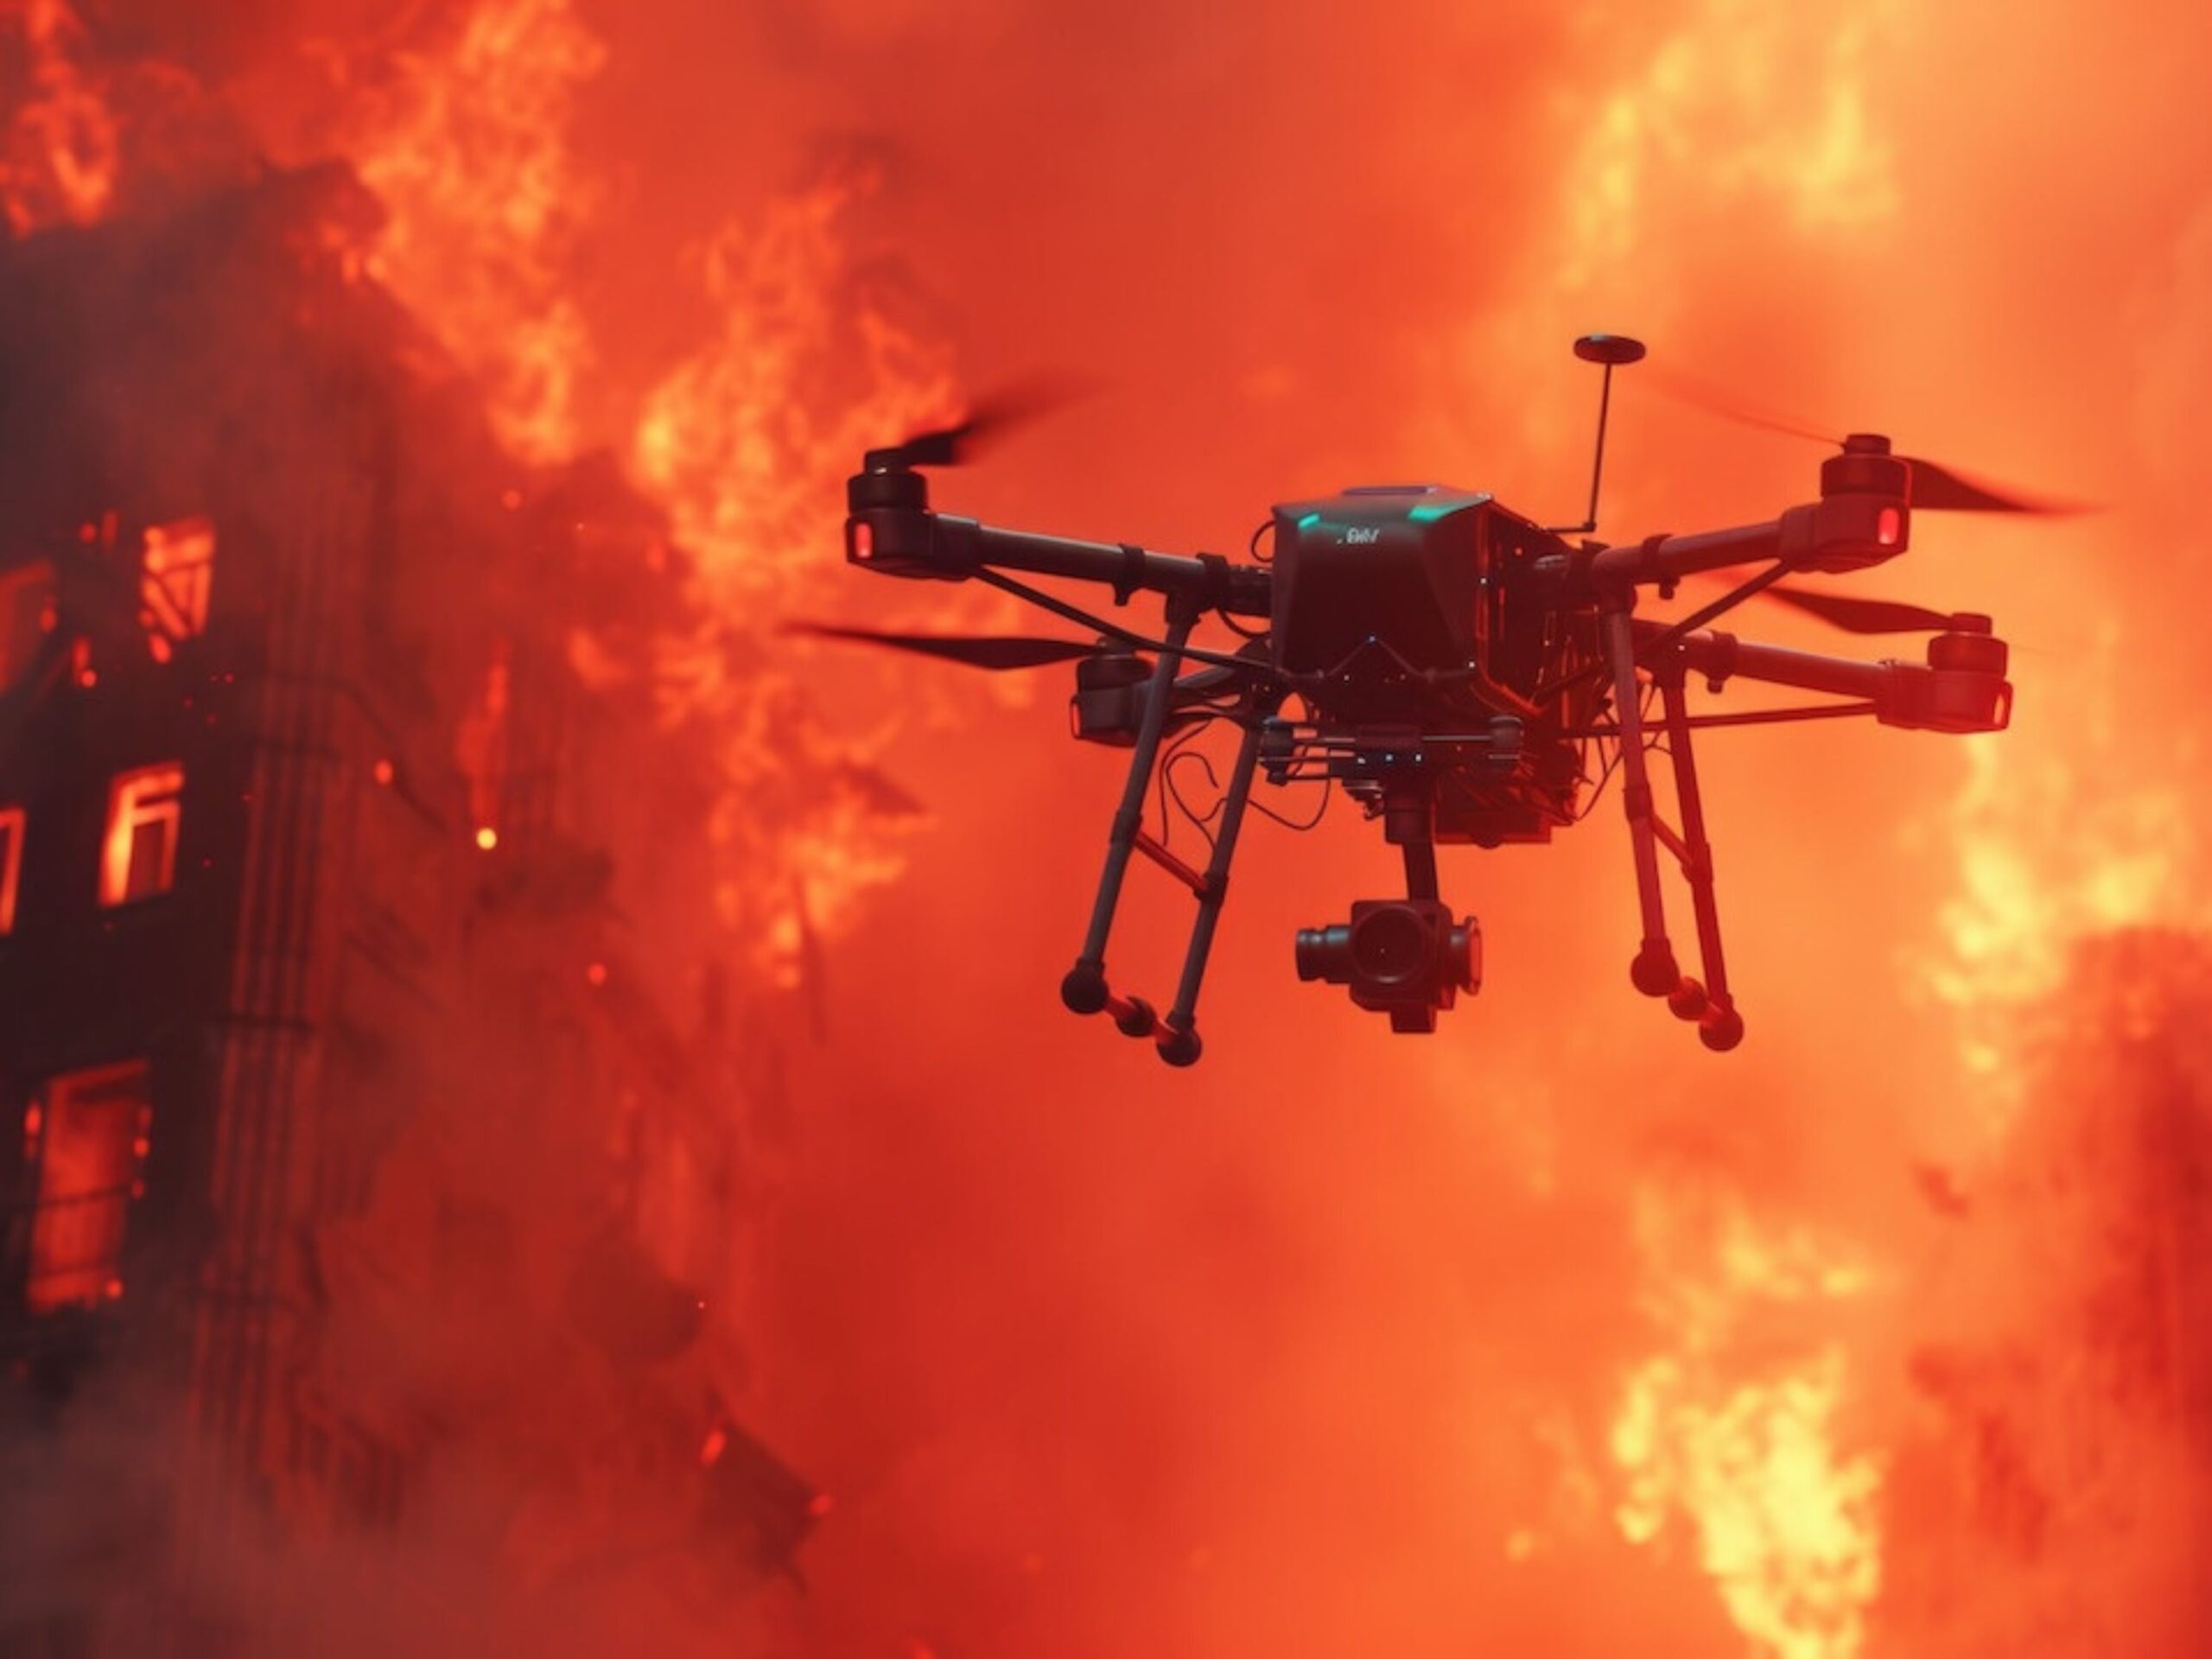
\includegraphics[width=0.95\textwidth]{images/drone_rescue.jpg}
    \vspace{0.2cm}
    {\footnotesize \textbf{Precision}}
    {\tiny Drone under stress}
  \end{columns}

  \vspace{0.5cm}

  {\tiny Guiard (1987): non-dominant hand is the \textbf{frame-setter}—it localizes position but \textit{not} fine motion. Without feedback, control is \textbf{impossible}.}
\end{frame}

% ====== SLIDE 3: BACKGROUND & MOTIVATION ======
\begin{frame}[plain]
  \vspace{0.5cm}
  \centering

  \textcolor{darkblue}{\Large \textbf{Why Feedback Channel Matters}}

  \vspace{0.5cm}

  \begin{tabular}{c c c}
    \textbf{No Feedback} & & \textbf{With Feedback} \\
    (Can't learn) & $\longrightarrow$ & (Brain adapts) \\
    \textcolor{red}{BLIND} & & \textcolor{darkblue}{$\checkmark$ AWARE}
  \end{tabular}

  \vspace{0.6cm}

  \textbf{\small Body Schema}

  {\small Maravita \& Iriki (2004): Brain extends into tools held in hand}

  \vspace{0.35cm}

  \textbf{\small Haptic Advantage}

  {\small Cuppone et al. (2016): Touch improves proprioceptive acuity}

  \vspace{0.35cm}

  \textbf{\small Audio Trade-off}

  {\small Sigrist et al. (2013): Sound may overload attention without clear mapping}

  \vspace{0.5cm}

  {\small \textit{Which channel helps non-dominant hand control?}}
\end{frame}

% ====== SLIDE 4: RESEARCH QUESTIONS (Baseline-Aware) ======
\begin{frame}[plain]
  \vspace{0.8cm}
  \centering

  \textcolor{darkblue}{\Large \textbf{Research Questions}}

  \vspace{0.6cm}

  \begin{tabular}{p{1.2cm} p{7.8cm}}
    \textbf{RQ1*} & Does modality affect fall counts? \\[0.3cm]
    \textbf{RQ2} & Does feedback improve performance (baseline-adjusted)? \\[0.3cm]
    \textbf{RQ3} & Which modality shows better improvement? \\[0.3cm]
    \textbf{RQ4} & Does difficulty interact with feedback? \\
  \end{tabular}

  \vspace{0.7cm}

  \fcolorbox{darkblue}{white}{%
    \parbox{0.9\textwidth}{%
      \centering
      \textbf{\textit{The Question:}} Does modality choice predict performance? \\
      \textbf{\textit{The Finding:}} Baseline and difficulty matter more.
    }
  }

  \vspace{0.5cm}

  {\tiny *Primary. RQ2–3 address the critical discovery: baseline control differs 10× by modality.}
\end{frame}

% ====== SLIDE 5: STUDY DESIGN (experimental setup) ======
\begin{frame}[plain]
  \vspace{0.6cm}
  \centering

  \textcolor{darkblue}{\Large \textbf{PathSense: Study Design}}

  \vspace{0.4cm}

  \begin{columns}[T]
    \column{0.45\textwidth}
    \centering
    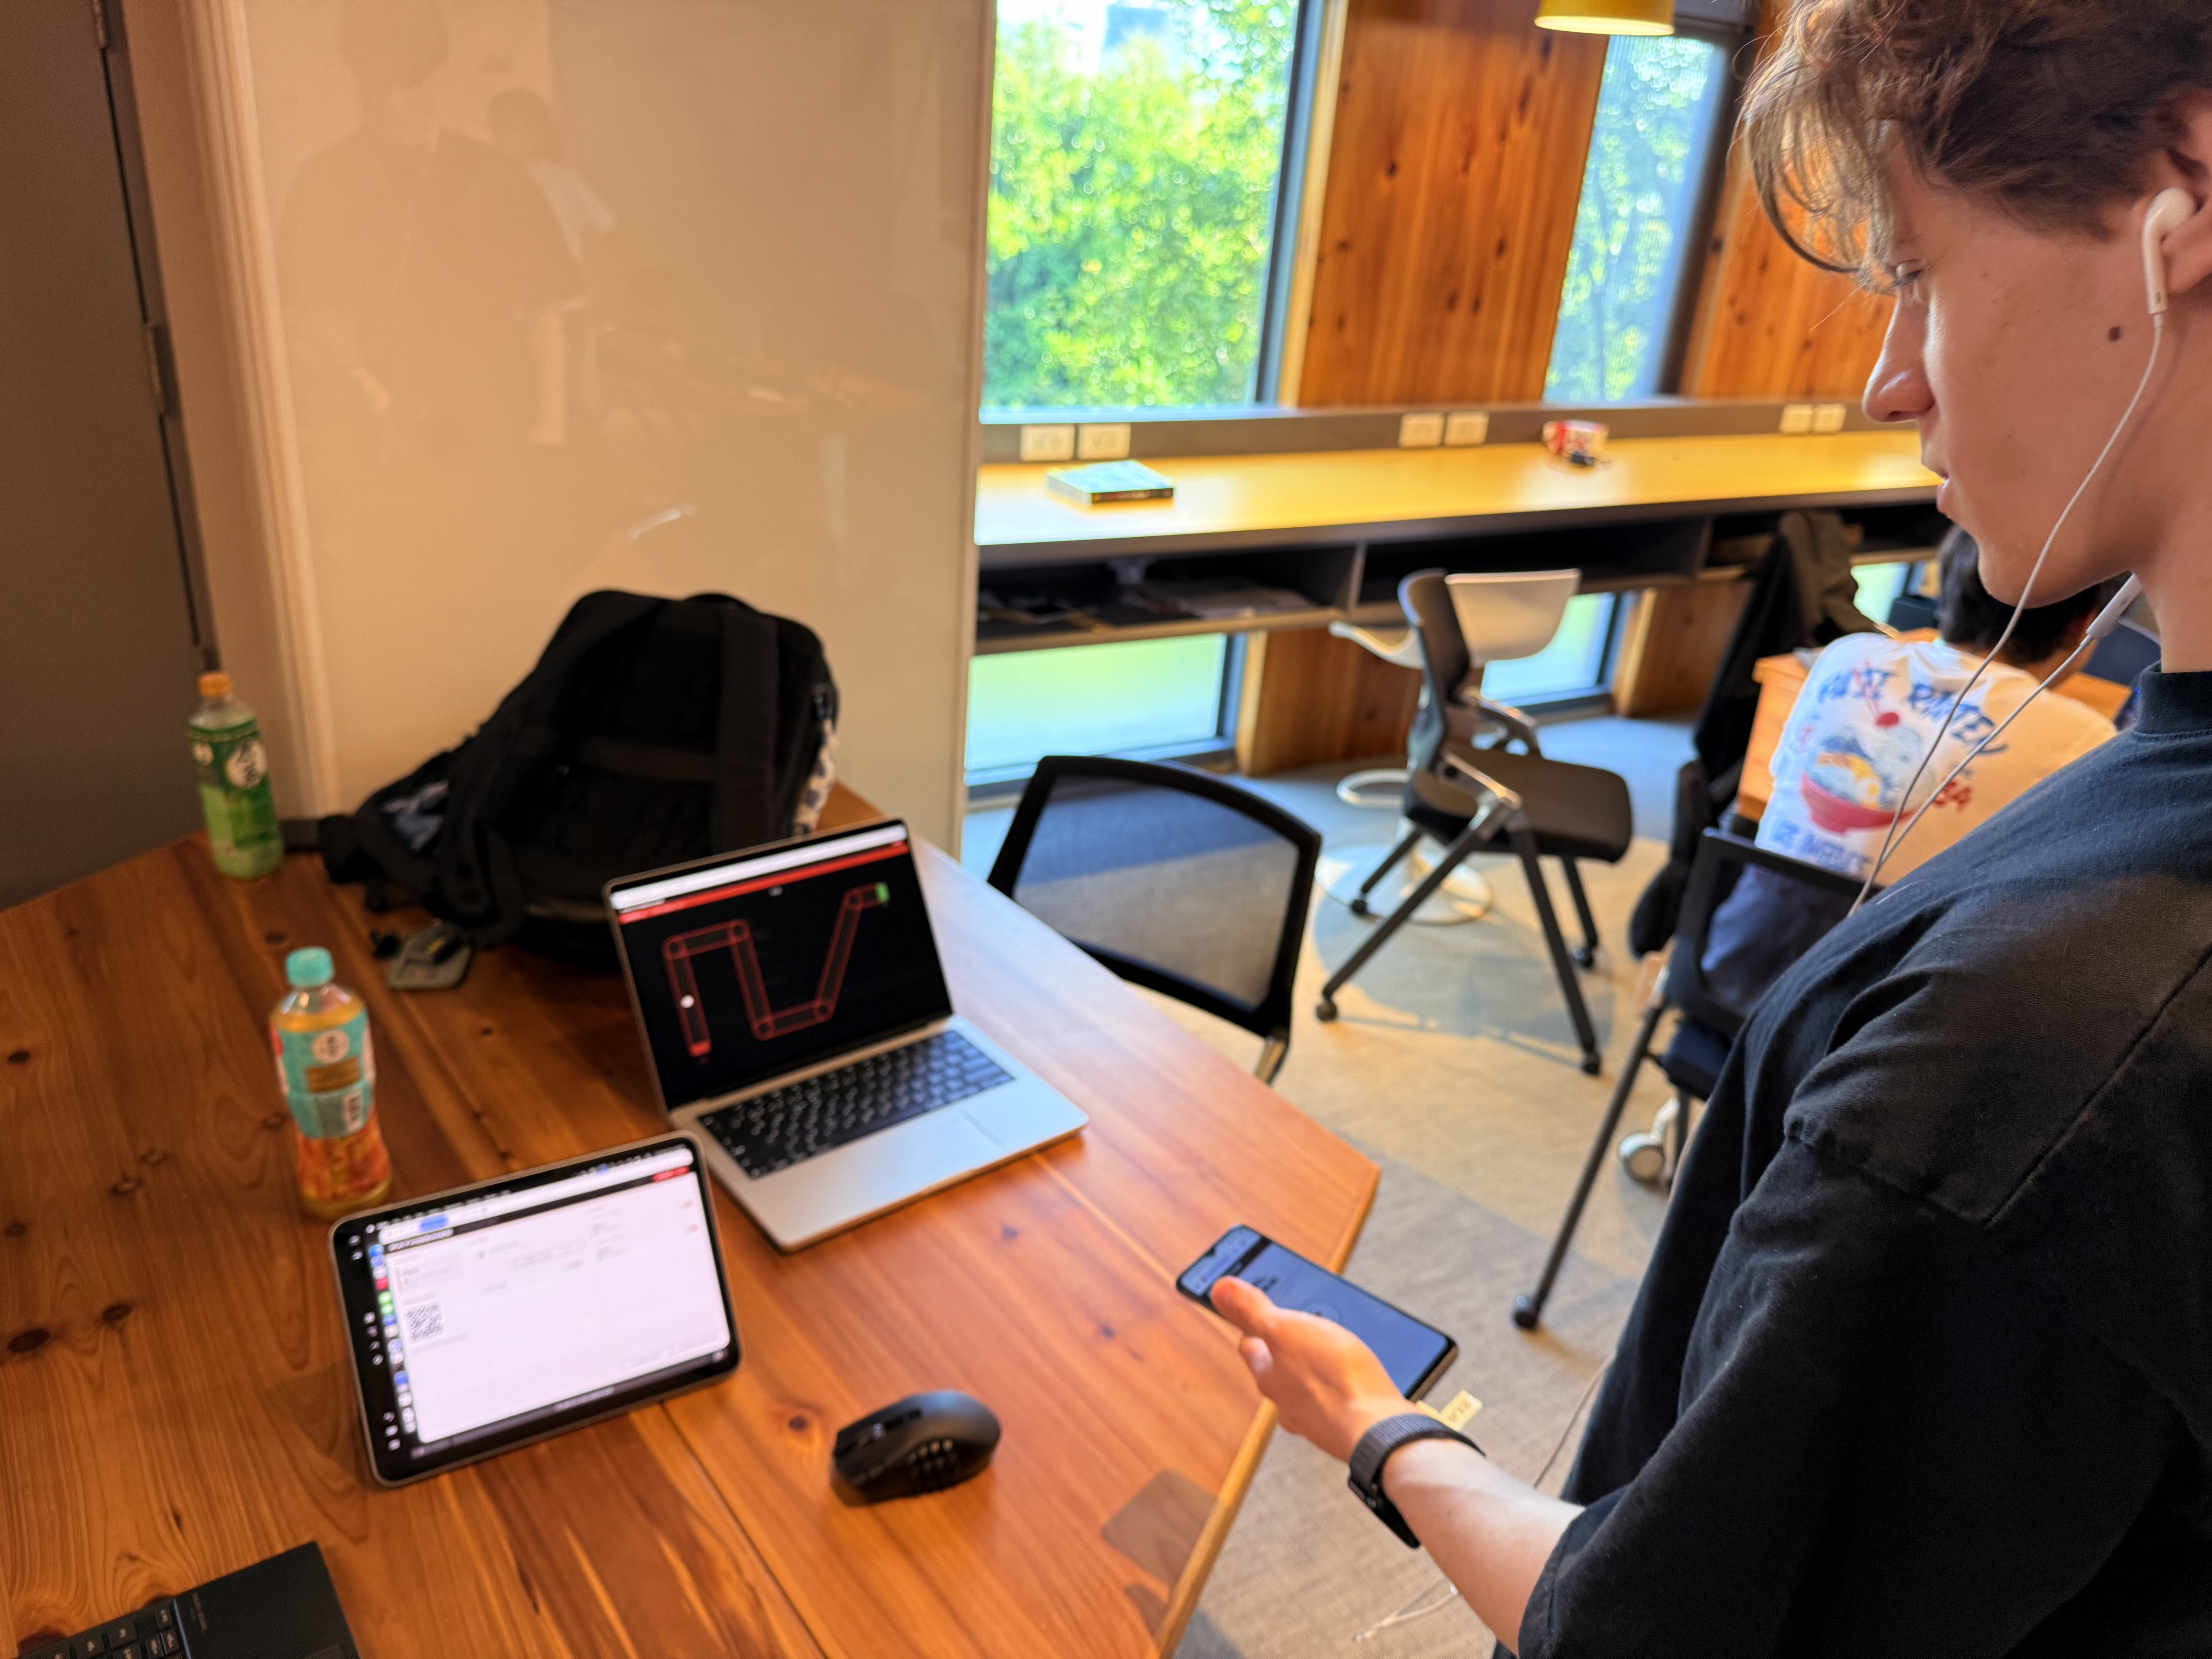
\includegraphics[width=0.92\textwidth]{images/pathsense_setup.jpeg}
    \vspace{0.2cm}
    {\tiny Participant + display + controller}

    \column{0.5\textwidth}
    \centering
    \textbf{\small Cohort Demographics}
    \vspace{0.2cm}

    \begin{tabular}{ll}
      \textbf{N} & 25 participants \\
      \textbf{Age} & 17.3 ± 5.2 yrs (13–47) \\
      \textbf{Gender} & 48\% M, 48\% W \\
      \textbf{Handedness} & 92\% right-handed \\
      \textbf{Modality} & 9 per condition \\
    \end{tabular}

    \vspace{0.4cm}

    \textbf{\small Difficulty Levels}

    {\tiny L1 Practice | L2 Easy | L3 Medium | L4 Hard}

    \vspace{0.3cm}

    \textbf{\small Measurement}

    {\tiny • Falls • Proximity • 10 Hz gyro}
  \end{columns}
\end{frame}

% ====== SLIDE 5a: THE THREE CONDITIONS ======
\begin{frame}[plain]
  \vspace{0.3cm}
  \centering

  \textcolor{darkblue}{\Large \textbf{The Three Feedback Conditions}}

  \vspace{0.2cm}

  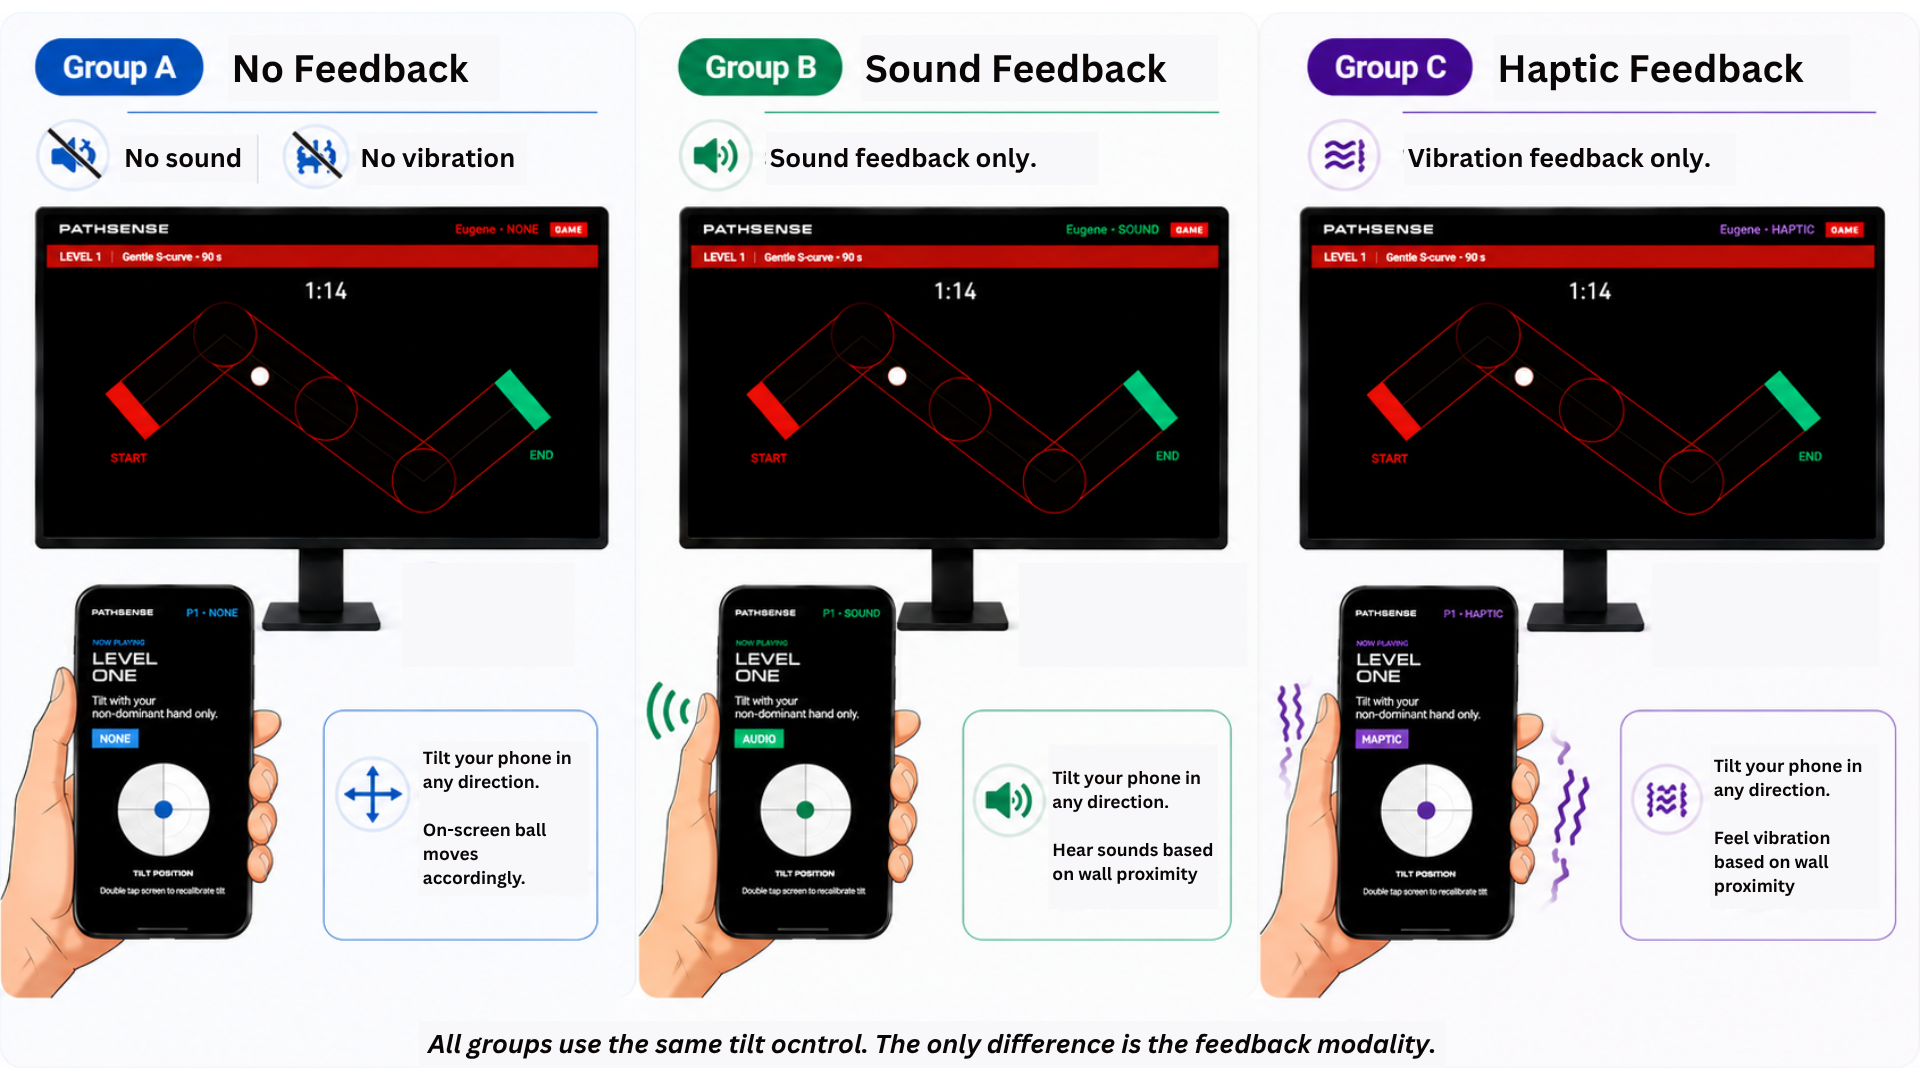
\includegraphics[width=0.98\textwidth]{images/three_conditions.png}

  \vspace{0.1cm}

  {\tiny All groups: same tilt control, same game, same difficulty levels. Only difference: feedback modality.}
\end{frame}

% ====== SLIDE 6: RESULTS — FALLS & PATH CONTROL ======
\begin{frame}[plain]
  \vspace{0.8cm}
  \centering

  \textcolor{darkblue}{\Large \textbf{Results: Control Accuracy \& Fall Rate}}

  \vspace{0.4cm}

  \begin{columns}[T]
    \column{0.5\textwidth}
    \centering
    {\small \textbf{Fall Counts}}
    \vspace{0.2cm}
    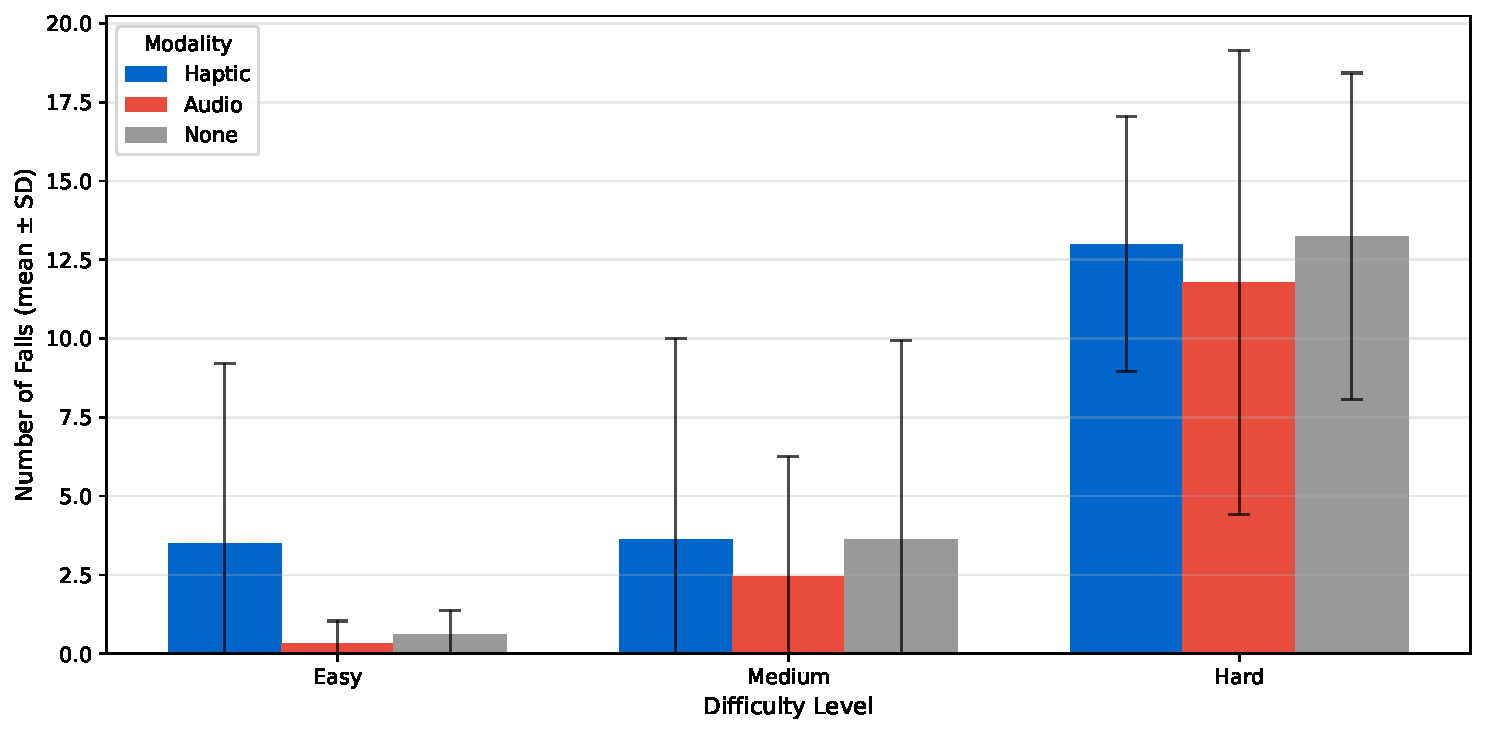
\includegraphics[width=0.95\textwidth]{fig_falls.pdf}

    \column{0.5\textwidth}
    \centering
    {\small \textbf{Path Deviation}}
    \vspace{0.2cm}
    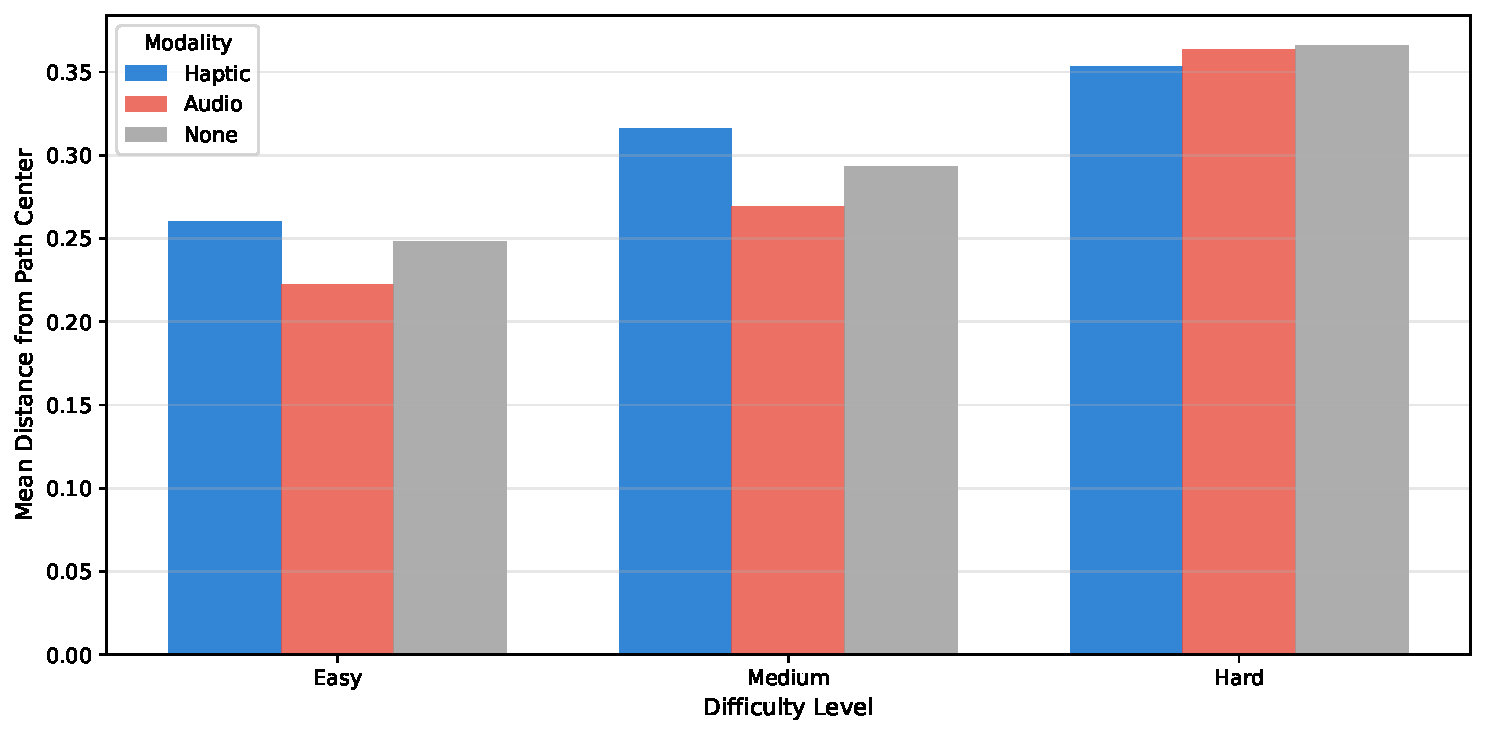
\includegraphics[width=0.95\textwidth]{fig_path_deviation.pdf}
  \end{columns}

  \vspace{0.2cm}

  {\tiny
    \textbf{RQ1 Statistics:}
    \begin{itemize}
      \item Kruskal-Wallis: $p > 0.19$ at all levels (L2–L4)
      \item Effect sizes (rank-biserial $r$): −0.44 to +0.25 (negligible)
      \item Mann-Whitney pairwise (Holm corrected): all $p > 0.27$
      \item Bayesian: $\text{BF}_{01} \approx 84$ (Easy), 7 (Medium), 5.4 (Hard)
      \item Sample sizes: $n=8$–$9$ per modality per level
    \end{itemize}
  }
\end{frame}

% ====== SLIDE 7: RESULTS — BASELINE CONFOUND & PROXIMITY ======
\begin{frame}[plain]
  \vspace{0.6cm}
  \centering

  \textcolor{darkblue}{\Large \textbf{Results: Baseline Confound \& Proximity Response}}

  \vspace{0.4cm}

  \begin{columns}[T]
    \column{0.42\textwidth}
    \centering
    {\small \textbf{Practice Baseline (Before Feedback)}}
    \vspace{0.4cm}

    \begin{tabular}{lc}
      \textbf{Group} & \textbf{Falls} \\
      \hline
      Audio & \textcolor{red}{0.33} $\checkmark$ \\
      None & 2.14 \\
      Haptic & \textcolor{darkblue}{4.88} $\times$ \\
    \end{tabular}

    \vspace{0.5cm}

    {\small \textcolor{red}{\textbf{10× gap}}}

    \vspace{0.2cm}

    {\tiny Groups unequal before testing}

    \column{0.55\textwidth}
    \centering
    {\small \textbf{Proximity Response (Stacked)}}
    \vspace{0.2cm}
    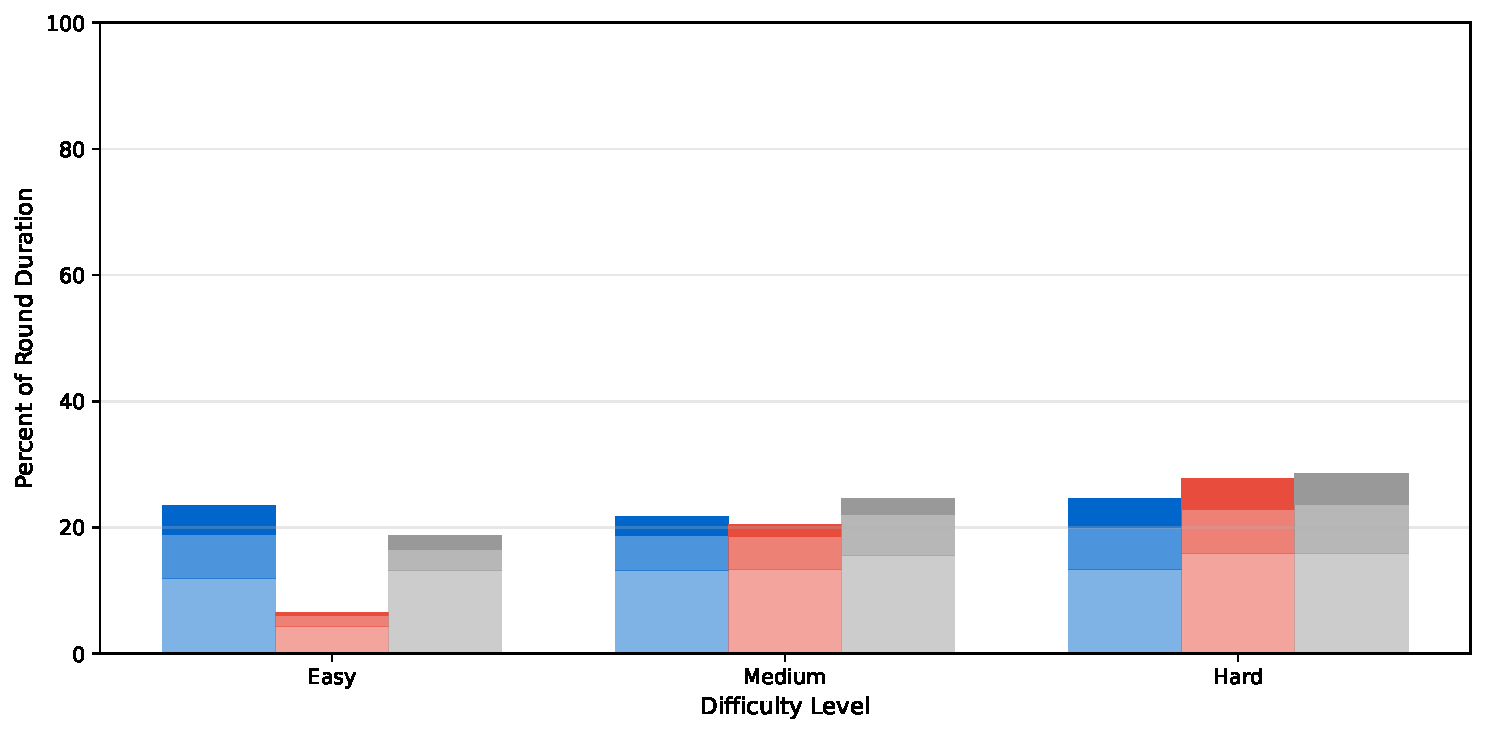
\includegraphics[width=0.98\textwidth]{fig_proximity_time.pdf}
    \vspace{0.15cm}
    {\tiny \textbf{Modalities:} \textcolor{darkblue}{Haptic} $|$ \textcolor{red}{Audio} $|$ \textcolor{darkgray}{None}} \\
    {\tiny \textbf{Zones:} Light (safe) | Medium (warn) | Dark (danger)}
  \end{columns}

  \vspace{0.15cm}

  {\tiny
    \textbf{Baseline Test (Practice):} Mann-Whitney $U = 28$, $p = 0.04$, $r = -0.57$ (moderate effect)

    \textbf{RQ2 (Change-from-baseline):} Haptic Δ = −1.38, Audio Δ = 0.00, None Δ = −2.38

    \textbf{RQ3:} Haptic shows relative improvement; audio flat. Small absolute differences.
  }
\end{frame}

% ====== SLIDE 8: RESULTS — LEARNING & STEERING RESPONSE ======
\begin{frame}[plain]
  \vspace{0.6cm}
  \centering

  \textcolor{darkblue}{\Large \textbf{Results: Learning Trajectory \& Steering Response}}

  \vspace{0.4cm}

  \begin{columns}[T]
    \column{0.5\textwidth}
    \centering
    {\small \textbf{Learning Curve}}
    \vspace{0.2cm}
    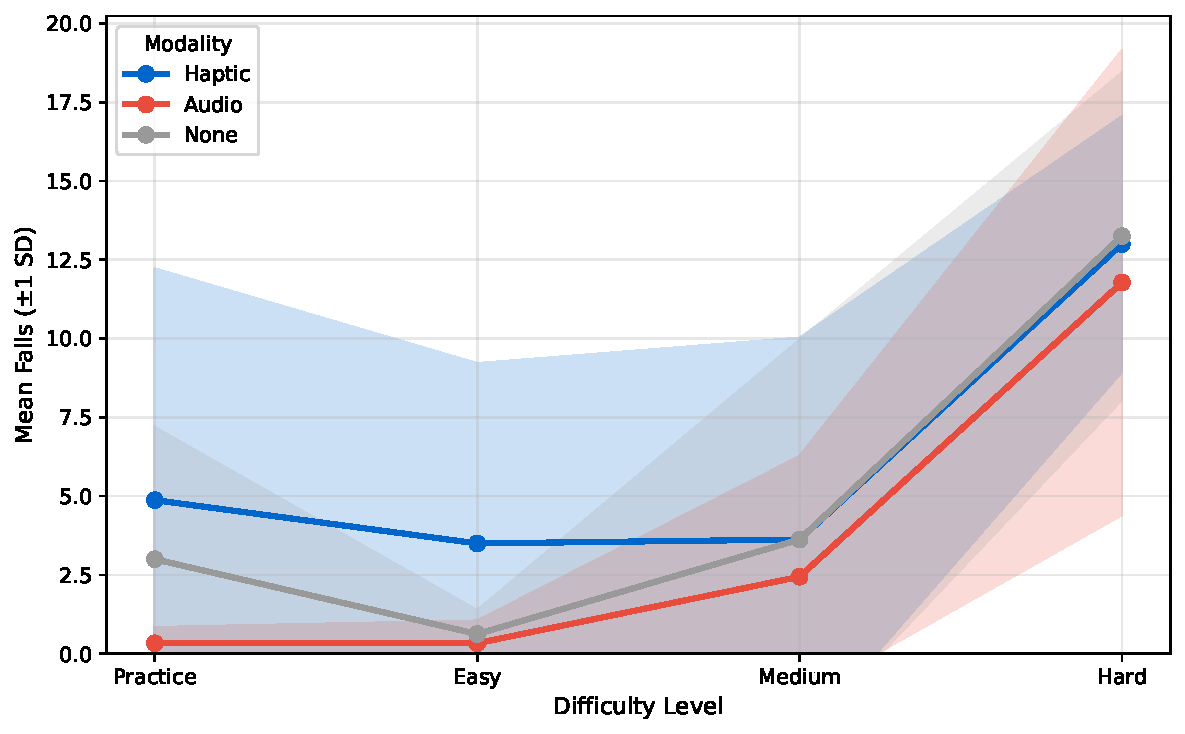
\includegraphics[width=0.98\textwidth]{fig_learning_curve.pdf}

    \column{0.5\textwidth}
    \centering
    {\small \textbf{Time-Locked Correction}}
    \vspace{0.2cm}
    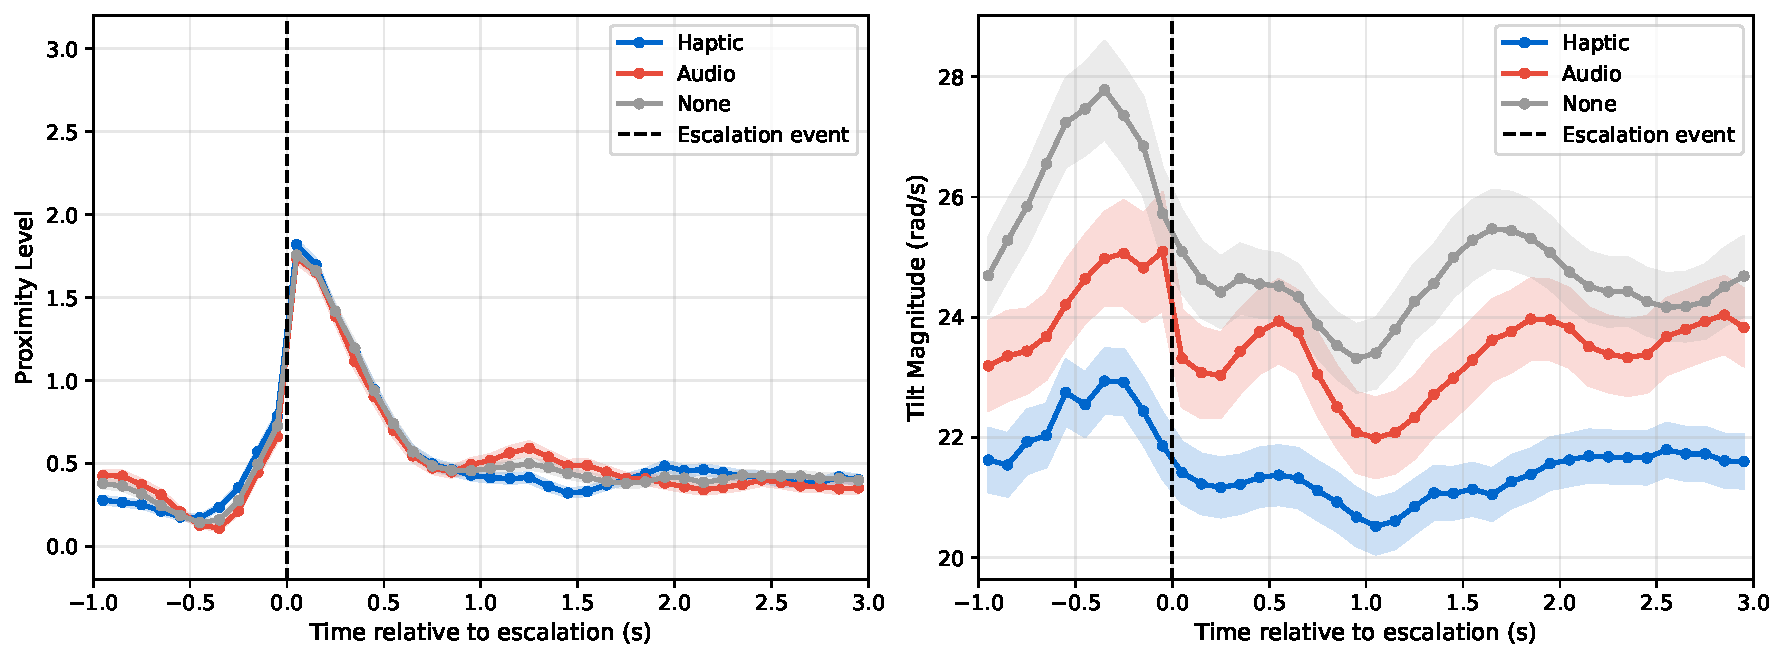
\includegraphics[width=0.98\textwidth]{fig_steering_response.pdf}
  \end{columns}

  \vspace{0.2cm}

  {\tiny
    \textbf{RQ4 (Difficulty × Modality):} All groups: improve at Easy (Δ ≈ −1 to −2 falls), deteriorate at Hard (Δ ≈ +8 to +11 falls). Kruskal-Wallis interaction test: $p > 0.19$.

    \textbf{Steering Response:} No modality advantage in time-to-recovery or correction magnitude. Difficulty is the dominant factor.
  }
\end{frame}

% ====== SLIDE 9: WHAT WE LEARNED ======
\begin{frame}[plain]
  \vspace{0.6cm}
  \centering

  \textcolor{darkblue}{\Large \textbf{What We Actually Found}}

  \vspace{0.6cm}

  \textbf{\small Finding 1: Baseline Varies Dramatically}

  {\tiny 10× gap in baseline control before any feedback. Groups weren't equal from start.}

  \vspace{0.4cm}

  \textbf{\small Finding 2: Modality Doesn't Predict Outcomes}

  {\tiny No modality effect at group level. Haptic ≠ Audio ≠ None (all p > 0.19). \\
  Bayesian analysis: $\text{BF}_{01} \approx 84$ (strong evidence for null).}

  \vspace{0.4cm}

  \textbf{\small Finding 3: Task Difficulty Dominates}

  {\tiny All groups improve at Easy, crash at Hard. Difficulty is the real limiter.}

  \vspace{0.5cm}

  \fcolorbox{darkblue}{white}{%
    \parbox{0.85\textwidth}{%
      \centering
      \small \textit{``It's a good training for elders or students with special needs.''} \\
      \tiny — Participant feedback (on audio condition)
    }
  }

  \vspace{0.3cm}

  {\tiny \textbf{Next step:} Individual-level analysis to understand responsiveness patterns.}
\end{frame}

% ====== SLIDE 10: CONCLUSION & KEY MESSAGE ======
\begin{frame}[plain]
  \vspace{0.6cm}
  \centering

  \textcolor{darkblue}{\Large \textbf{What We Learned}}

  \vspace{0.6cm}

  {\small
    \begin{tabular}{ll}
      RQ1: & No modality effect on absolute falls \\
      RQ2/RQ3: & Baseline responsiveness predicts improvement \\
      RQ4: & Task difficulty, not feedback, dominates \\
    \end{tabular}
  }

  \vspace{0.8cm}

  \fcolorbox{darkblue}{white}{%
    \parbox{0.85\textwidth}{%
      \centering
      \small \textbf{This study said "No" to modality.} \\
      \small \textit{But that "No" led to a better question:} \\
      \small \textbf{\textit{Who IS responsive to which feedback?}}
    }
  }

  \vspace{0.6cm}

  {\tiny
    \textbf{Next:} Scale sample. Test more populations. Continue building. \\
    \textbf{Insight:} Measure baseline first. It predicts everything. \\[0.2cm]
    \textbf{Refs:} Guiard (1987) • Maravita \& Iriki (2004) • Cuppone et al. (2016)
  }
\end{frame}

\end{document}
